\chapter{Morfologisk analyse af kontrolsystem} \label{Bilag - morf til kontrolsystem}

Kontrolsystemet til det mekaniske koncept der ses i figur \ref{fig:Endelig mekaniske koncept} findes ved at lave en morfologisk analyse med delfunktionerne til kontrolsystemet fra funktionstræet i figur \ref{Figur: Funktionstræ}. Der er identificeret to delfunktioner til kontrolsystemet; \textit{brugerflade} og \textit{Kalibrering af emne placering}, som der udarbejdes delkoncepter til. Delkoncepterne samles til konceptforslag, der sættes sammen med det mekaniske koncept. Til den første delfunktion er der fundet 4 delkoncepter, som er følgende: \plainbreak{0.5}
\paragraph{Knapper og skærm}
Knapper og skærm monteres på robotten og agerer som styresystem, hvor man kan starte og stoppe prikoverapplikationen, følge processen af prikapplikationen samt finjustere faktorer som prikstørrelse ved brug af knapperne.

\paragraph{Touchskærm}
Touchskærmen vil fungere med samme udgangspunkt som knapper og skærm, med forskel at alt interaktion med robotten sker gennem touchskærmen og ikke med knapper.

\paragraph{Knapper}
Knapperne benyttes til alt interaktion med robotten, hvorved der ikke gøres brug af en skærm. Dette begrænser den information der kan videregives brugeren, og betyder dermed at variable informationer som tid tilbage eller fejl vil være svære at oversætte. Dette betyder at det er brugerens ansvar at oversætte disse situationer.

\paragraph{Ekstern computer}
Tilslutning af en ekstern computer tillader alt information vist på egen computer, hvilket betyder at et tilslutningskabel og software er nødvendigt for at maskinen kan køre.
\plainbreak{1}

Til kalibrering af emne placeringer er der fundet følgende 5 delkoncepter: \plainbreak{0.5}
\paragraph{Laser}
En eller flere photon senor, vil blive opsat og sende lys ud, som robotten kan bruge ved at måle forskellen i tid det tager fra der udsendes lys til at det modtages igen. Robotten vil finde afstanden til emnet ud fra hvor lang tid lys rejser på den pågældende tid lyset var udsendt.

\paragraph{Kontakt med emnet}
Robotten vil køre rundt i arbejdsområdet, indtil den kommer i kontakt med emnet og følge emnets form rundt. Robotten vil huske hvilken bane den har kørt og dermed markere dette som emnet.

\paragraph{Sensor der påsættes}
Sensorer vil i dette tilfælde blive påsat på emnets hjørner, som vil sende deres position til robotten, som bruger disse informationer til at danne et arbejdsområde. Når sensorerne fjernes, beholder robotten positionsinformationerne og bruger dem til at prikke det korrekte område.

\paragraph{Indtast på computer}
Emnets form og dimensioner indtastes på en computer, hvorefter dataene sendes til robotton, som dermed bruger informationerne til at sætte prikker de rigtige steder. 
%Emnet har nogle mål, som i dette tilfælde vil blive indtastet på en computer. Disse mål vil derefter blive sendt til robotten, dermed ved robotten hvor emnet befinder sig.

\paragraph{Kamera} 
Et kamera monteres over prikemnet, som vil fotografere emnet i xy-planet og sende det til robotten, hvor prikemnet findes ved at vurdere forskellen på lys i baggrund og ved prikemnet. \plainbreak{1}

Delkoncepterne er indsat i tabel \ref{tab: morfologisk analyse af kontrolsystem}, hvor konceptforslag er markeret ved forskellige former og farver. 


\begin{table}[H]
    \caption{Morfologisk analyse af kontrolsystemet. 1 $=$ \protect\lillacirc, 2 $=$ \protect\bluebox, 3 $=$ \protect\cyanbox, 4 $=$ \protect\blueangle, 5 $=$ \protect\greenangle, 6 $=$ \protect\gulangle, 7 $=$ \protect\orangeangle, 8 $=$ \protect\pinkstar, 9 $=$ \protect\redkant, 10 $ = \protect\mathcolor{BrickRed}{\clubsuit}$, 11 $=$ \protect\lillacircny, 12 $=$ \protect\blueboxny, 13 $=$ \protect\cyanboxny, 14 $=$ \protect\blueangleny, 15 $=$ \protect\greenangleny, 16 $=$ \protect\gulangleny, 17 $=$ \protect\orangeangleny, 18 $=$ \protect\pinkstarny, 19 $=$ \protect\redkantnyy \ og 20 $= \protect\mathcolor{BrickRed}{\spadesuit}$}
    \centering
    \begin{tabular}{|l|p{2.5cm}|p{2.61cm}|p{2.61cm}|p{2.61cm}|p{2.61cm}|} \cline{2-6}   
    %% Title
        \multicolumn{1}{l|}{} & \multicolumn{5}{|c|}{\cellcolor{aaublue} \textcolor{white}{\textbf{Delkoncepter til kontrolsystem delfunktioner}}} \\ \cline{2-6}
    %% Headers
        \multicolumn{1}{l|}{}  & \multicolumn{1}{c|}{ \cellcolor{lightgray!20} \textbf{1}} & \multicolumn{1}{|c|}{\cellcolor{lightgray!20} \textbf{2}} & \multicolumn{1}{c|}{\cellcolor{lightgray!20} \textbf{3}} & \multicolumn{1}{c|}{\cellcolor{lightgray!20} \textbf{4}} & \multicolumn{1}{c|}{\cellcolor{lightgray!20} \textbf{5}} \\ \cline{2-6} \specialrule{0pt}{0.5pt}{0pt}
    %Pictures
        \rotatebox[origin=c]{90}{\cellcolor{aaublue} \textcolor{white}{\textbf{Brugerflade}}} & \makecell{ Knapper \\ og skærm \\ \includegraphics[width=.98\linewidth]{Sections/5 Konceptgenerering/Media/Knapper og skærm.png} \\ \lillacirc \ \bluebox \ \cyanbox \ \blueangle \ \greenangle } & \makecell{Knapper \\ \includegraphics[width=.98\linewidth]{Sections/5 Konceptgenerering/Media/knapper.png} \\ \gulangle \ \orangeangle \ \pinkstar \ \redkant \  $ \protect\mathcolor{BrickRed}{\clubsuit}$} & \makecell{ Ekstern \\ computer\\ 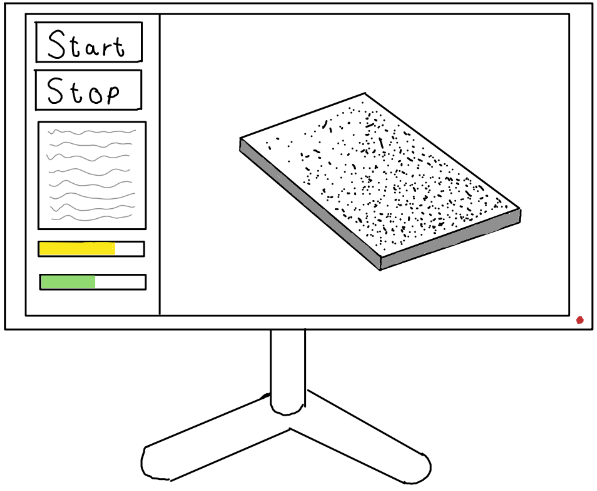
\includegraphics[width=.98\linewidth]{Sections/5 Konceptgenerering/Media/Computer.png} \\ \lillacircny \ \blueboxny \ \cyanboxny \ \blueangleny \ \greenangleny} & \makecell{Touch \\  skærm \\ \includegraphics[width=.98\linewidth]{Sections/5 Konceptgenerering/Media/Touch skærm.png} \\ \gulangleny \ \orangeangleny \ \pinkstarny \ \redkantnyy \ $ \protect\mathcolor{BrickRed}{\spadesuit}$}  &  \\ \specialrule{1pt}{0pt}{0pt}

        %Formanalyse af emne
        \rotatebox[origin=c]{90}{\cellcolor{aaublue} \textcolor{white}{\textbf{Kalibrering af emne placering}}} & \makecell{Laser \\ 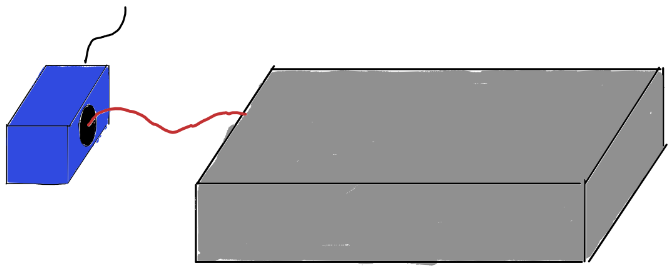
\includegraphics[width=0.98\linewidth]{Sections/5 Konceptgenerering/Media/Laser.png} \\ \lillacirc \ \gulangle \ \lillacircny \ \gulangleny} & \makecell{Kamera \\ 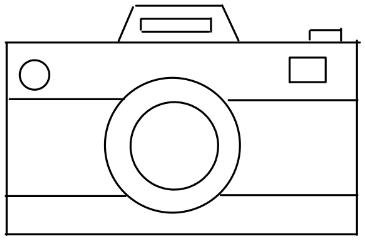
\includegraphics[width=0.8\linewidth]{Sections/5 Konceptgenerering/Media/Kamera.png} \\ \bluebox \ \orangeangle \ \blueboxny \ \orangeangleny} & \makecell{ Kontakt \\ med emnet \\ 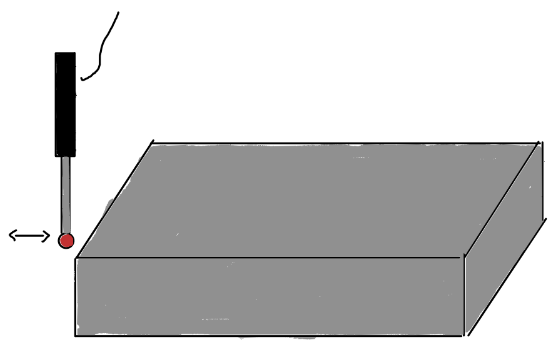
\includegraphics[width=0.98\linewidth]{Sections/5 Konceptgenerering/Media/Kontakt.png} \\ \cyanbox \ \pinkstar \ \cyanboxny \ \pinkstarny} & \makecell{Indtast på \\ computer \\ 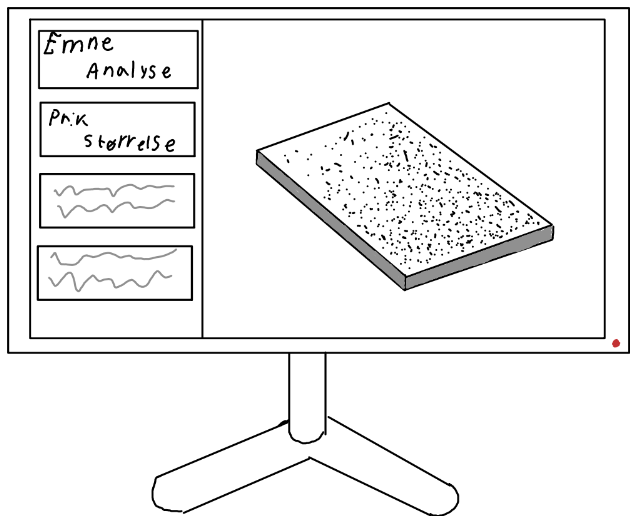
\includegraphics[width=0.98\linewidth]{Sections/5 Konceptgenerering/Media/formanalyse compu.png} \\ \blueangle \ \redkant \ \blueangleny \ \redkantnyy} & \makecell{Sensor der \\ påsættes \\ 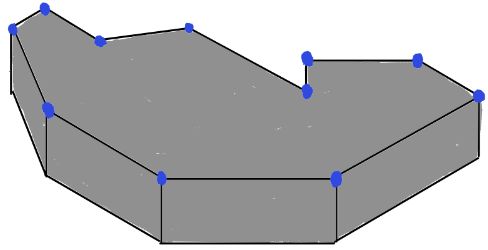
\includegraphics[width=0.98\linewidth]{Sections/5 Konceptgenerering/Media/sensor i punkt.png} \\ \greenangle \ $\protect\mathcolor{BrickRed}{\clubsuit}$ \ \greenangleny \ $\protect\mathcolor{BrickRed}{\spadesuit}$ }  \\ \specialrule{1pt}{0pt}{0pt}
 
    \end{tabular}
    \label{tab: morfologisk analyse af kontrolsystem}
\end{table}



\section{Konceptforslag til kontrolsystem} \label{Konceptforlag - kontrolsystem}

Det er muligt at lave alle 20 konceptforlag, idet ingen delkoncepter er indbyrdes inkompatible, i modsætning til delkoncepterne til de mekaniske dele i afsnit \ref{Bilag - morf til kontrolsystem}. Konceptforslag til kontrolsystemet fra tabel \ref{tab: morfologisk analyse af kontrolsystem}. Alle konceptforslagene vurderes i et screening skema i afsnit \ref{Kontrolsystem - vurdering}.




\section{Screening af koncepter til kontrolsystem} \label{Kontrolsystem - vurdering}
De 20 konceptforslag til kontrolsystemet fra den morfologiske analyse i afsnit \ref{Bilag - morf til kontrolsystem} gennemgårs ved et screening skema. Screening skemaet er udført på samme måde som for de mekaniske dele i afsnit \ref{Mekanisk system - vurdering}, ved at hver delløsning blev vurderet i forhold til opstillede vurderingskriterier baseret ønsker og designspecifikationer fra kapitel \ref{Konceptgenerering}. Hvert konceptforslags vurdering er summen af point fra de enkelte delkoncepter som konceptforslaget er samlet af. Delkoncepterne i konceptforslag 1 er referencepunktet, som de øvrige delkoncepter vurderes ud fra. 

Hvert vurderingskriterie fik tildelt en vægt i form af et heltal fra 1-4, for at klargøre hvilket kriterie der er vigtigst. Vægtene er baseret på baggrund af vægtningerne fra kundens ønsker, samt designspecifikationer fra HoQ i kap. \ref{Kravspecifikation}.


\begin{table}[H]
    \centering
    \scriptsize
    \caption{screening skema. Koncepternes værdier til de forskellige kriterier, er summen af værdier fra et koncepts delløsninger. Vægtningen af hvert vurderingskriterie er angivet med "V" og ses i kolonnen længst til højre.}
    \begin{tabular}{|p{2cm}|c c c c c c c c c c c|} \cline{2-10}

        \multicolumn{1}{c}{}& \multicolumn{10}{|c|}{\cellcolor{aaublue} \small \textcolor{white}{\textbf{Konceptforslag til kontrolsystem}}} \\ \hline
         
        \multicolumn{1}{|c|}{\cellcolor{lightgray!20}\textbf{Vurderingskriterier}} & \multicolumn{1}{c||}{\cellcolor{lightgray!20}\textbf{1} \protect\lillacirc}  &\multicolumn{1}{c}{\cellcolor{lightgray!20}\textbf{2 \protect\bluebox}} &\multicolumn{1}{c}{\cellcolor{lightgray!20}\textbf{3 \protect\cyanbox}} &\multicolumn{1}{c}{\cellcolor{lightgray!20}\textbf{4 \protect\blueangle}} &\multicolumn{1}{c}{\cellcolor{lightgray!20}\textbf{5 \protect\greenangle}} &\multicolumn{1}{c}{\cellcolor{lightgray!20}\textbf{6 \protect\gulangle}}  &\multicolumn{1}{c}{\cellcolor{lightgray!20}\textbf{7 \protect\orangeangle}} &\multicolumn{1}{c}{\cellcolor{lightgray!20}\textbf{8 \protect\pinkstar}} &\multicolumn{1}{c}{\cellcolor{lightgray!20}\textbf{9 \protect\redkant}} &\multicolumn{1}{c}{\cellcolor{lightgray!20}\textbf{10 $\protect\mathcolor{BrickRed}{\clubsuit}$}} &\multicolumn{1}{||r|}{\cellcolor{lightgray!20}\textbf{V}} \\ \hline
         
    %% Vurdering
        % Hurtighed/tid i processen
         \multicolumn{1}{|l|}{\cellcolor{aaublue} \textcolor{white}{\scriptsize \textbf{Hurtighed/tid i processen}}} 
         & \multicolumn{1}{c||}{0} & 0 & -1 & -1 & -2 & -1 & -1 & -2 & -2 & -3 & \multicolumn{1}{||c|}{3}\\ \hline
        % Brugervenlighed  
         \multicolumn{1}{|l|}{\cellcolor{aaublue} \textcolor{white}{\scriptsize \textbf{Brugervenlighed}}} 
         & \multicolumn{1}{c||}{0} & 0 & 0 & -1 & -2 & 0 & 0 & 0 & -1 & -2 & \multicolumn{1}{||c|}{4} \\ \hline
        % Holdbarhed
         \multicolumn{1}{|l|}{\cellcolor{aaublue} \textcolor{white}{\scriptsize \textbf{Holdbarhed}}} 
         & \multicolumn{1}{c||}{0} & 0 & -1 & 0 & -1 & 1 & 1 & 0 & 1 & 0 & \multicolumn{1}{||c|}{2} \\\hline
        % Kompleksitet af Fremstilling
         \multicolumn{1}{|l|}{\cellcolor{aaublue} \textcolor{white}{\scriptsize\textbf{Kompleksitet ved fremstilling}}} 
         & \multicolumn{1}{c||}{0} & 0 & -1 & 0 & 0 & 1 & 1 & 0 & 1 & 1 & \multicolumn{1}{||c|}{1} \\\hline
        % Kompleksitet af Samling
         \multicolumn{1}{|l|}{\cellcolor{aaublue} \textcolor{white}{\scriptsize\textbf{Kompleksitet ved samling}}} 
         & \multicolumn{1}{c||}{0} & 1 & 0 & 1 & 0 & 0 & 1 & 0 & 1 & 0 & \multicolumn{1}{||c|}{2} \\\hline
        % Forskellige emne former
         \multicolumn{1}{|l|}{\cellcolor{aaublue} \textcolor{white}{\scriptsize \textbf{Forskellige emne former}}} 
         & \multicolumn{1}{c||}{0} & 1 & -1 & 0 & -1 & 0 & 1 & -1 & 0 & -1 & \multicolumn{1}{||c|}{3} \\\hline
%% Samlet score og rank
        \specialrule{0pt}{2pt}{0pt} \cline{1-11}
        \multicolumn{1}{|r|}{\cellcolor{lightgray!10} \textbf{Samlet score}}& \multicolumn{1}{c||}{0} & 2 & -4 & -1 & -6 & 1 & 3 & -3 & 0 & -5 & \multicolumn{1}{|c}{} \\\cline{1-11}
        
        \multicolumn{1}{|r|}{\cellcolor{lightgray!10} \textbf{Vægtet score}}& \multicolumn{1}{c||}{0} & 5 & -9 & -5 & -19 & 0 & 5 & -9 & -5 & -19 &\multicolumn{1}{|c}{} \\\cline{1-11} 

        \multicolumn{1}{|r|}{\cellcolor{lightgray!10}\textbf{Rangering}}& \multicolumn{1}{c||}{7} & 3 & 15 & 11 & 19 & 7 &  3 & 15 & 11 & 19 & \multicolumn{1}{|c}{} \\\cline{1-11}

 
%% 11-20
        \specialrule{0pt}{5pt}{0pt} \hline
        \multicolumn{1}{|c|}{\cellcolor{lightgray!20}\textbf{Vurderingskriterier}} & \multicolumn{1}{c}{\cellcolor{lightgray!20}\textbf{11 \protect\lillacircny}}  &\multicolumn{1}{c}{\cellcolor{lightgray!20}\textbf{12 \protect\blueboxny}} &\multicolumn{1}{c}{\cellcolor{lightgray!20}\textbf{13 \protect\cyanboxny}} &\multicolumn{1}{c}{\cellcolor{lightgray!20}\textbf{14 \protect\blueangleny}} &\multicolumn{1}{c}{\cellcolor{lightgray!20}\textbf{15 \protect\greenangleny}} &\multicolumn{1}{c}{\cellcolor{lightgray!20}\textbf{16 \protect\gulangleny}} &\multicolumn{1}{c}{\cellcolor{lightgray!20}\textbf{17 \protect\orangeangleny}} &\multicolumn{1}{c}{\cellcolor{lightgray!20}\textbf{18 \protect\pinkstarny}} &\multicolumn{1}{c}{\cellcolor{lightgray!20}\textbf{19 \protect\redkantnyy}} &\multicolumn{1}{c}{\cellcolor{lightgray!20}\textbf{20 $\protect\mathcolor{BrickRed}{\spadesuit}$}} & \multicolumn{1}{||r|}{\cellcolor{lightgray!20}\textbf{V}} \\ \hline
         
%% Vurdering
        % Hurtighed/tid i processen
         \multicolumn{1}{|l|}{\cellcolor{aaublue} \textcolor{white}{\textbf{\scriptsize Hurtighed/tid i processen}}} 
         & 0 & 0 & -1 & -1 & -2 & 1 & 1 & 0 & 0 & -1 & \multicolumn{1}{||c|}{3} \\ \hline
        % Brugervenlighed  
         \multicolumn{1}{|l|}{\cellcolor{aaublue} \textcolor{white}{\scriptsize \textbf{Brugervenlighed}}} 
         & 0 & 0 & 0 & -1 & -2 & 0 & 0 & 0 & -1 & -2 & \multicolumn{1}{||c|}{4} \\ \hline
        % Holdbarhed
         \multicolumn{1}{|l|}{\cellcolor{aaublue} \textcolor{white}{\scriptsize \textbf{Holdbarhed}}} 
         & 1 & 1 & 0 & -1 & -2 & 0 & 0 & 0 & -1 & -2 & \multicolumn{1}{||c|}{2} \\\hline
        % Kompleksitet af Fremstilling
         \multicolumn{1}{|l|}{\cellcolor{aaublue} \textcolor{white}{\scriptsize \textbf{Kompleksitet ved fremstilling}}} 
         & 0 & 0 & -1 & 0 & 0 & 1 & 1 & 0 & 1 & 1 & \multicolumn{1}{||c|}{1} \\\hline
        % Kompleksitet af Samling
         \multicolumn{1}{|l|}{\cellcolor{aaublue} \textcolor{white}{\scriptsize \textbf{Kompleksitet ved samling}}} 
         & 1 & 2 & 1 & 2 & 1 & 0 & 1 & 0 & 1 & 0 & \multicolumn{1}{||c|}{2} \\\hline
        % Forskellige emne former
         \multicolumn{1}{|l|}{\cellcolor{aaublue} \textcolor{white}{\scriptsize \textbf{Forskellige emne former}}} 
         & 0 & 1 & -1 & 0 & -1 & 0 & 1 & -1 & 0 & -1 & \multicolumn{1}{||c|}{3} \\\hline
         \specialrule{0pt}{2pt}{0pt} \cline{1-11}
%% Samlet score og rank
        \multicolumn{1}{|r|}{\cellcolor{lightgray!10} \textbf{Samlet score}}& 2 & 4 & -2 & 1 & -4 & 1 & 3 & -3 & 0 & \multicolumn{1}{c}{-5} & \multicolumn{1}{|c}{} \\\cline{1-11}
        
        \multicolumn{1}{|r|}{\cellcolor{lightgray!10} \textbf{Vægtet score}}& 4 & 9 & -5 & -1 & -15 & 2 & 7 & -7 & -3 & \multicolumn{1}{c}{-17} &\multicolumn{1}{|c}{} \\\cline{1-11} 
        
        \multicolumn{1}{|r|}{\cellcolor{lightgray!10}\textbf{Rangering}} & 5 & \multicolumn{1}{c}{\cellcolor{OliveGreen} \textcolor{white}{\textbf{1}}} & 11 & 9 & 17 & 6 &  \multicolumn{1}{c}{\cellcolor{OliveGreen} \textcolor{white}{\textbf{2}}} & 14 & 10 & \multicolumn{1}{c}{18} & \multicolumn{1}{|c}{} \\\cline{1-11}
    \end{tabular}
    \label{tab:selektionsskema kontrolsystem}
\end{table}
\plainbreak{1}
Screeningen af kontrolsystemet resulterede i at koncept 12 og 17, var de to topkandidater. Begge koncepter gør brug af et kamera til kalibrering af emne placering, og adskiller sig derved fra brugerfladen. Koncept 12 gør brug af en ekstern computer, som brugeren selv medbringer, hvorimod koncept 17 gør brug af en touch skærm. Det er vurderet at en løsning, der ikke kræver at brugeren skal en computer med en bestemt software, vil være et mere brugervenligt produkt. Denne vurdering har resulteret i, at koncept 17 er blevet valgt som det endelige kontrolsystem koncept.






\section{Vurdering af kontrolsystem dele}



\begin{figure}[H]
    \centering
    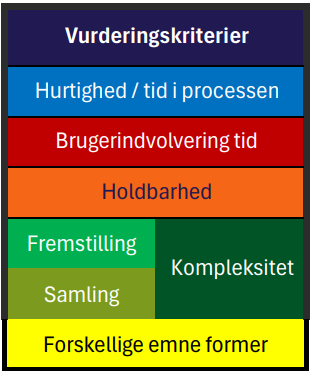
\includegraphics[width=0.25\linewidth]{bilag/Media/Media/delkoncept kontrol beskrivelse.png}
\end{figure}

\begin{figure}[H]
    \centering
    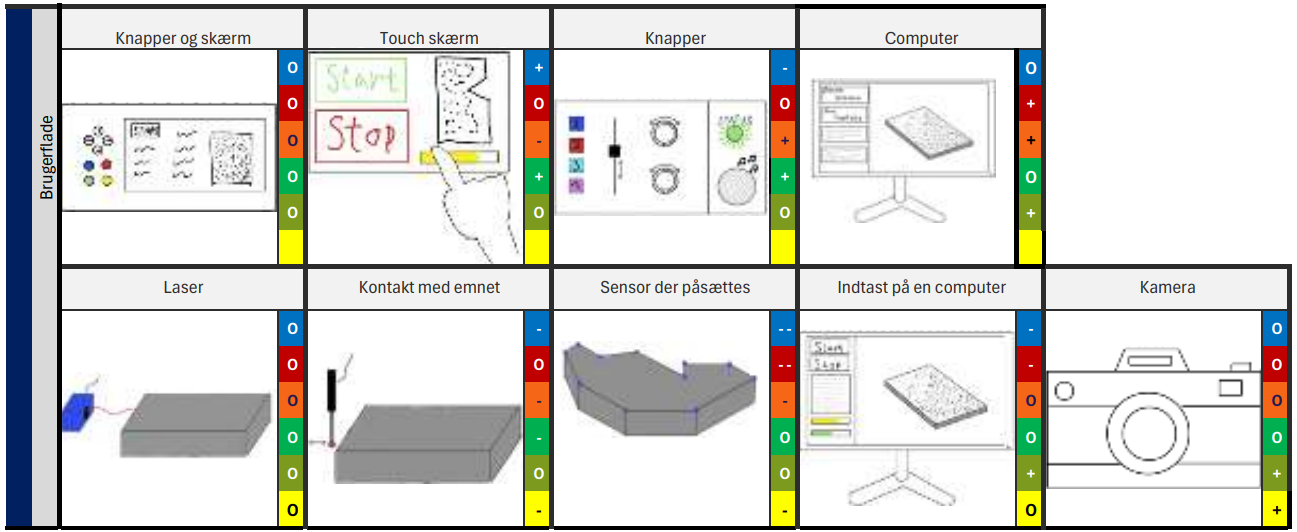
\includegraphics[width=1\linewidth]{bilag/Media/Media/delkoncept kontrol.png}
\end{figure}


\begin{table}[H]
    \centering
    \begin{tabular}{|p{0.4cm}|p{3.7cm}|p{2.4cm}| c |p{0.4cm}|p{3.7cm}|p{2.4cm}|} \cline{1-3} \cline{5-7}
        \multicolumn{1}{|p{0.4cm}|}{\cellcolor{aaublue} \textcolor{white}{Nr.}} &  \multicolumn{1}{|p{3.7cm}|}{\cellcolor{aaublue} \textcolor{white}{ Kalibrering af emne placering}} &  \multicolumn{1}{|p{2.4cm}|}{\cellcolor{aaublue} \textcolor{white}{ Brugerflade}} &  &  \multicolumn{1}{|p{0.4cm}|}{\cellcolor{aaublue} \textcolor{white}{Nr.}} &   \multicolumn{1}{|p{3.7cm}|}{\cellcolor{aaublue} \textcolor{white} {Kalibrering af emne placering}}  &  \multicolumn{1}{|p{2.4cm}|}{\cellcolor{aaublue} \textcolor{white}{Brugerflade}} \\ \cline{1-3} \cline{5-7}
    
        1 & \makecell{\includegraphics[width=0.8\linewidth]{Sections/5 Konceptgenerering/Media/Knapper og skærm.png}} & \makecell{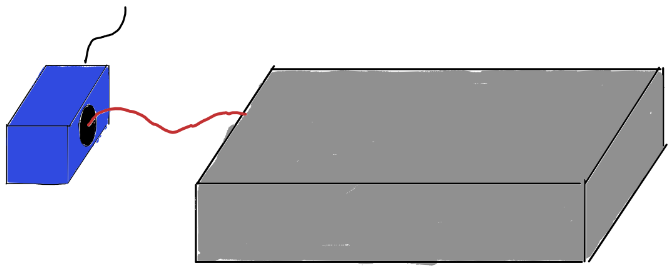
\includegraphics[width=0.98\linewidth]{Sections/5 Konceptgenerering/Media/Laser.png}} &   & 6 & \makecell{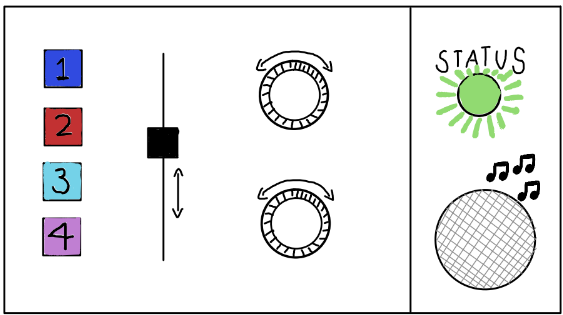
\includegraphics[width=0.8\linewidth]{Sections/5 Konceptgenerering/Media/Knapper.png}} & \makecell{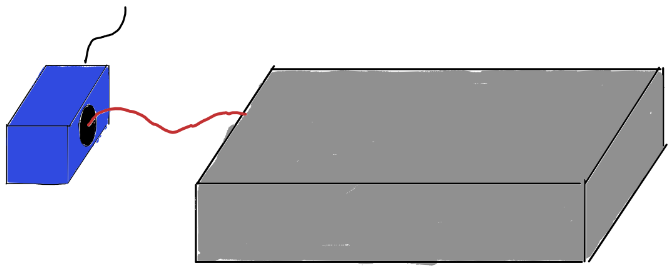
\includegraphics[width=0.98\linewidth]{Sections/5 Konceptgenerering/Media/Laser.png}}  \\ \cline{1-3} \cline{5-7}

        2 & \makecell{\includegraphics[width=0.8\linewidth]{Sections/5 Konceptgenerering/Media/Knapper og skærm.png}} & \makecell{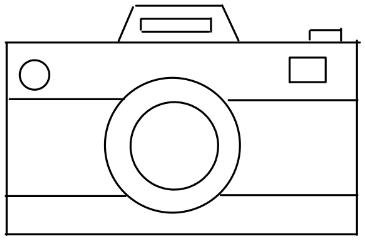
\includegraphics[width=0.98\linewidth]{Sections/5 Konceptgenerering/Media/Kamera.png}} &   &   7 & \makecell{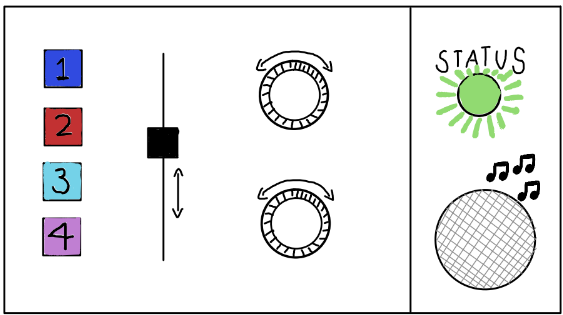
\includegraphics[width=0.8\linewidth]{Sections/5 Konceptgenerering/Media/Knapper.png}} & \makecell{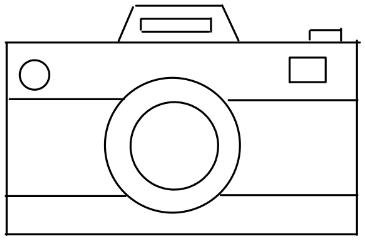
\includegraphics[width=0.98\linewidth]{Sections/5 Konceptgenerering/Media/Kamera.png}} \\ \cline{1-3} \cline{5-7}

        3 & \makecell{\includegraphics[width=0.8\linewidth]{Sections/5 Konceptgenerering/Media/Knapper og skærm.png}} & \makecell{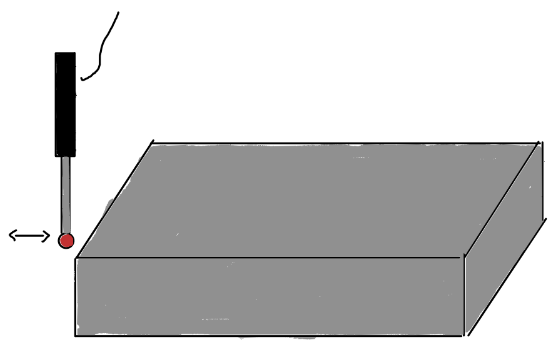
\includegraphics[width=0.98\linewidth]{Sections/5 Konceptgenerering/Media/Kontakt.png}} &   & 8 & \makecell{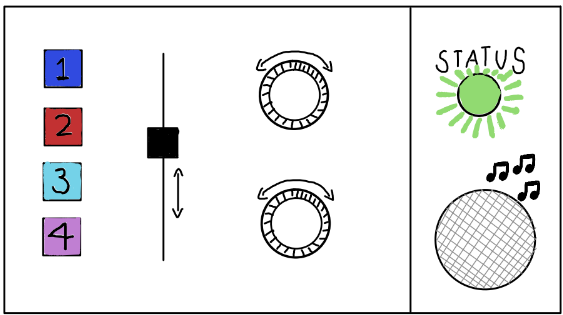
\includegraphics[width=0.8\linewidth]{Sections/5 Konceptgenerering/Media/Knapper.png}} & \makecell{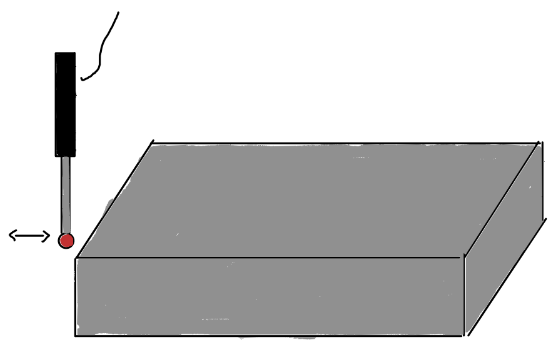
\includegraphics[width=0.98\linewidth]{Sections/5 Konceptgenerering/Media/Kontakt.png}} \\ \cline{1-3} \cline{5-7}

        4 & \makecell{\includegraphics[width=0.7\linewidth]{Sections/5 Konceptgenerering/Media/Knapper og skærm.png}} & \makecell{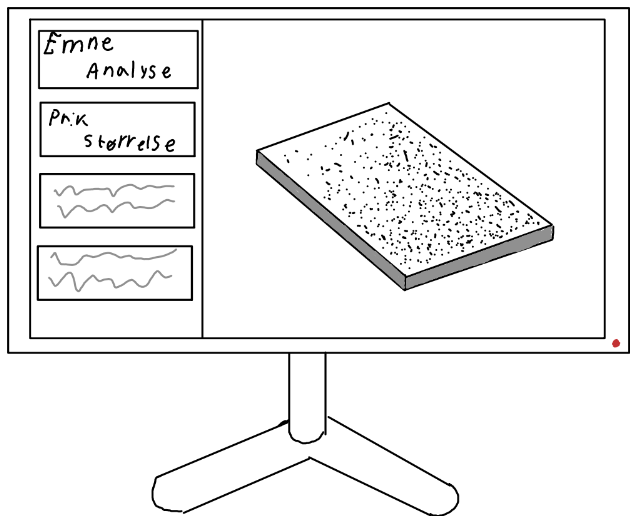
\includegraphics[width=0.98\linewidth]{Sections/5 Konceptgenerering/Media/formanalyse compu.png}} &   & 9 & \makecell{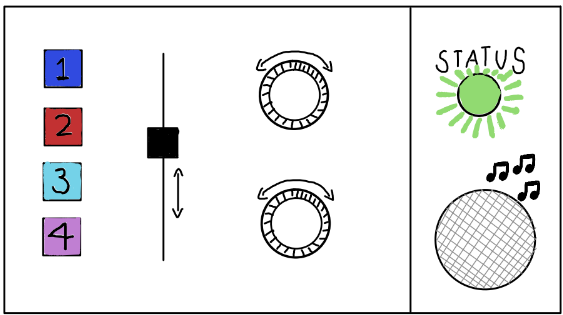
\includegraphics[width=0.7\linewidth]{Sections/5 Konceptgenerering/Media/Knapper.png}} & \makecell{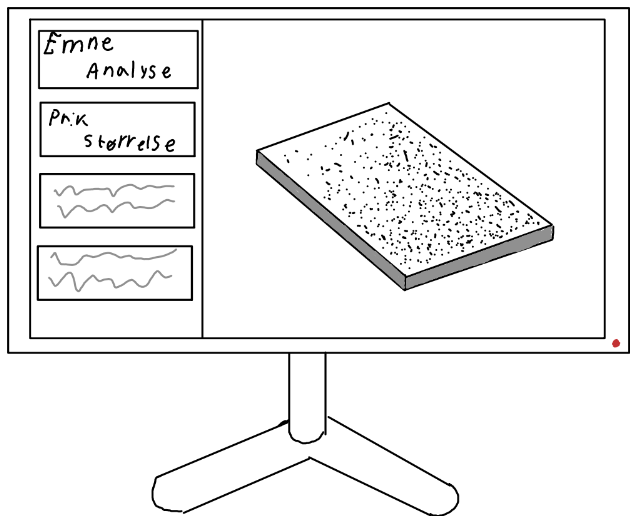
\includegraphics[width=0.98\linewidth]{Sections/5 Konceptgenerering/Media/formanalyse compu.png}}  \\ \cline{1-3} \cline{5-7}

        5 & \makecell{\includegraphics[width=0.8\linewidth]{Sections/5 Konceptgenerering/Media/Knapper og skærm.png}} & \makecell{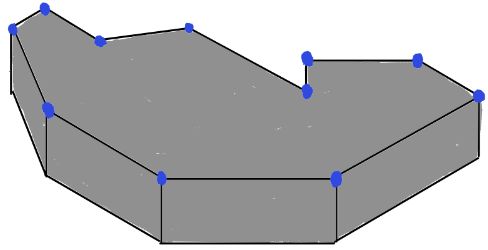
\includegraphics[width=0.98\linewidth]{Sections/5 Konceptgenerering/Media/sensor i punkt.png}} &   & 10 & \makecell{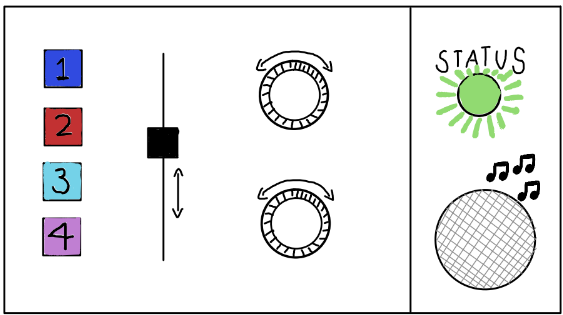
\includegraphics[width=0.8\linewidth]{Sections/5 Konceptgenerering/Media/Knapper.png}} & \makecell{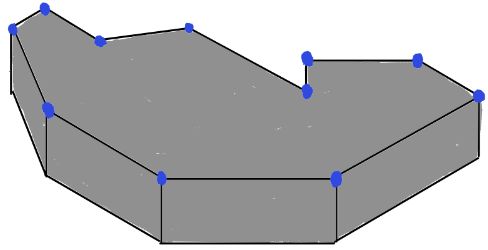
\includegraphics[width=0.98\linewidth]{Sections/5 Konceptgenerering/Media/sensor i punkt.png}}  \\ \cline{1-3} \cline{5-7}
    \end{tabular}
\end{table}

Tabel fortsættes på næste side.
I de næste tabeller er hvert delkoncept vurderet i forhold til relevante krav, som det ses i tabellen over. 0 betyder at delkonceptet hverken opfylder eller besværliggør opfyldelsen af et krav. + betyder at delkonceptet opfylder kravet eller gør det nemmere for løsningen at gøre det. - betyder at delkonceptet ikke opfylder eller besværliggør opfyldelsen af et krav. -- betyder at delkonceptet betydeligt besværliggør eller slet ikke opfylder et krav.
Herunder er alle konceptsammensætninger vurderet i forhold til deres delkomponenters opfyldelse af krav. Den sammensætning med højest vurdering i forhold til kravene og deres vigtighed vil blive brugt i løsningen. Dette er touch-skærmen og kameraet som det ses i figur \ref{tab:selektionsskema kontrolsystem}.




\begin{table}[H]
    \centering
    \begin{tabular}{|p{0.4cm}|p{3.7cm}|p{2.4cm}| c |p{0.4cm}|p{3.7cm}|p{2.4cm}|} \cline{1-3} \cline{5-7}
        \multicolumn{1}{|p{0.4cm}|}{\cellcolor{aaublue} \textcolor{white}{Nr.}} &  \multicolumn{1}{|p{3.7cm}|}{\cellcolor{aaublue} \textcolor{white}{Kalibrering af emne placering}} &  \multicolumn{1}{|p{2.4cm}|}{\cellcolor{aaublue} \textcolor{white}{ Brugerflade}} &  &  \multicolumn{1}{|p{0.4cm}|}{\cellcolor{aaublue} \textcolor{white}{Nr.}} &   \multicolumn{1}{|p{3.7cm}|}{\cellcolor{aaublue} \textcolor{white} {Kalibrering af emne placering}}  &  \multicolumn{1}{|p{2.4cm}|}{\cellcolor{aaublue} \textcolor{white}{Brugerflade}} \\ \cline{1-3} \cline{5-7}
        
        
        11 & \makecell{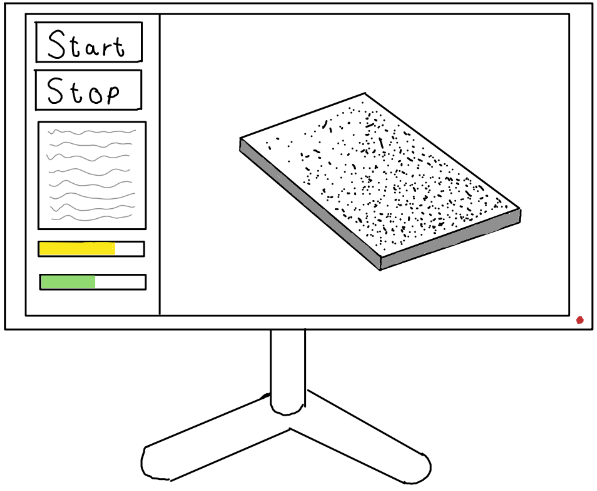
\includegraphics[width=0.7\linewidth]{Sections/5 Konceptgenerering/Media/Computer.png}} & \makecell{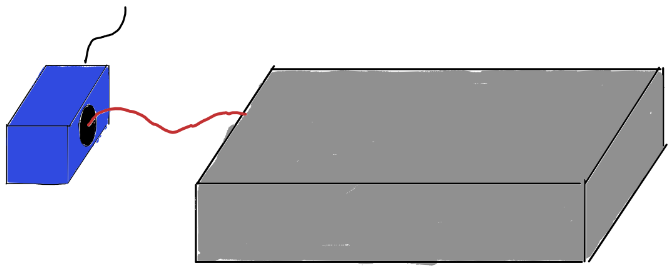
\includegraphics[width=0.98\linewidth]{Sections/5 Konceptgenerering/Media/Laser.png}} &   & 16 & \makecell{\includegraphics[width=0.7\linewidth]{Sections/5 Konceptgenerering/Media/Touch skærm.png}} & \makecell{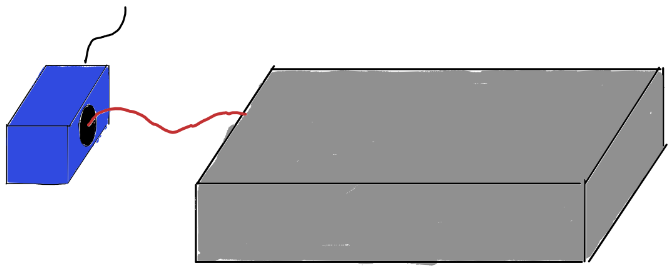
\includegraphics[width=0.98\linewidth]{Sections/5 Konceptgenerering/Media/Laser.png}}  \\ \cline{1-3} \cline{5-7}

       12 & \makecell{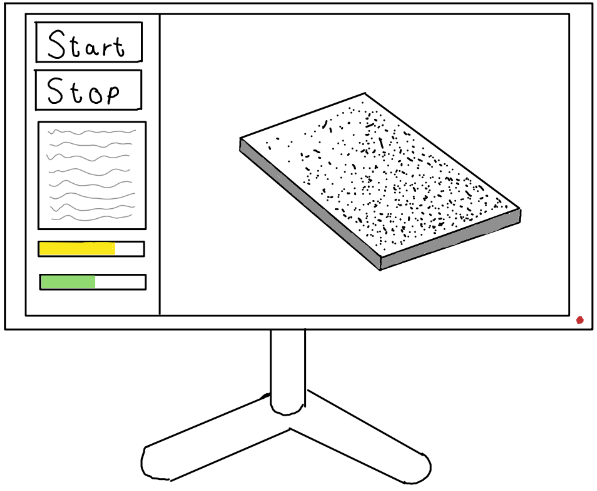
\includegraphics[width=0.7\linewidth]{Sections/5 Konceptgenerering/Media/Computer.png}} & \makecell{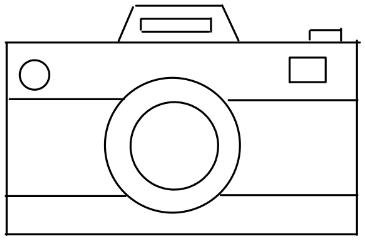
\includegraphics[width=0.98\linewidth]{Sections/5 Konceptgenerering/Media/Kamera.png}} &   & 17 & \makecell{\includegraphics[width=0.7\linewidth]{Sections/5 Konceptgenerering/Media/Touch skærm.png}} & \makecell{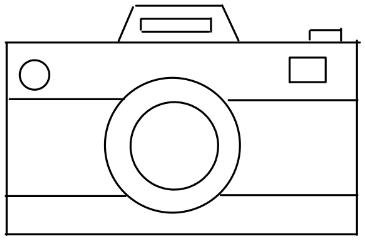
\includegraphics[width=0.98\linewidth]{Sections/5 Konceptgenerering/Media/Kamera.png}}  \\ \cline{1-3} \cline{5-7}

        13 & \makecell{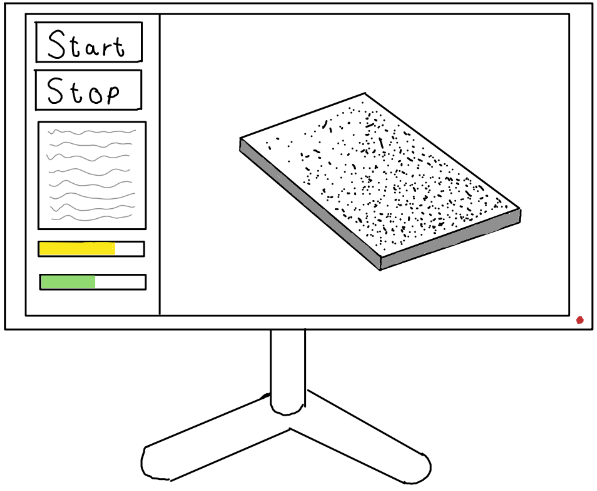
\includegraphics[width=0.7\linewidth]{Sections/5 Konceptgenerering/Media/Computer.png}} & \makecell{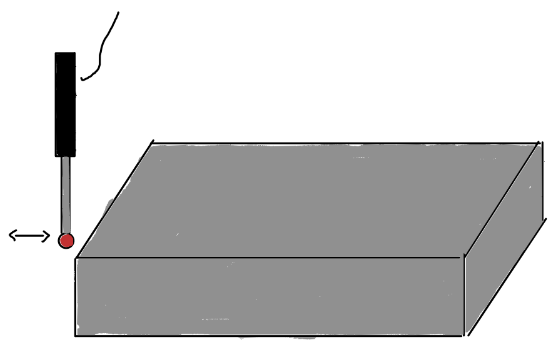
\includegraphics[width=0.98\linewidth]{Sections/5 Konceptgenerering/Media/Kontakt.png}} &   & 18 & \makecell{\includegraphics[width=0.7\linewidth]{Sections/5 Konceptgenerering/Media/Touch skærm.png}} & \makecell{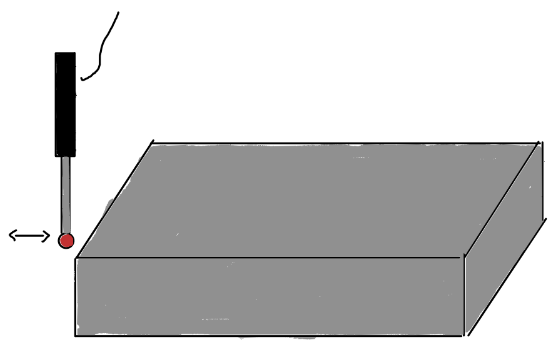
\includegraphics[width=0.98\linewidth]{Sections/5 Konceptgenerering/Media/Kontakt.png}}  \\ \cline{1-3} \cline{5-7}

        14 & \makecell{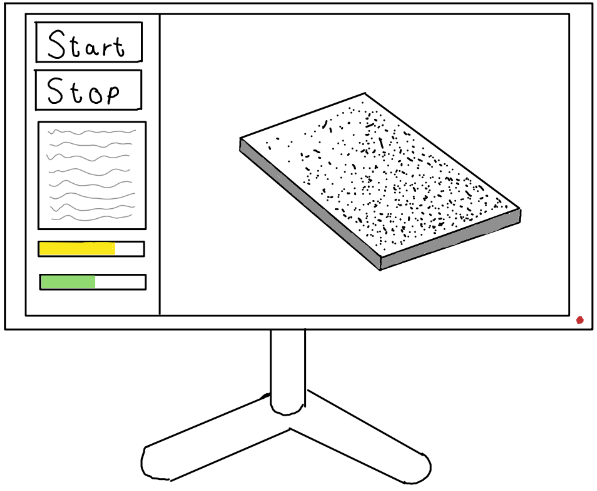
\includegraphics[width=0.7\linewidth]{Sections/5 Konceptgenerering/Media/Computer.png}} & \makecell{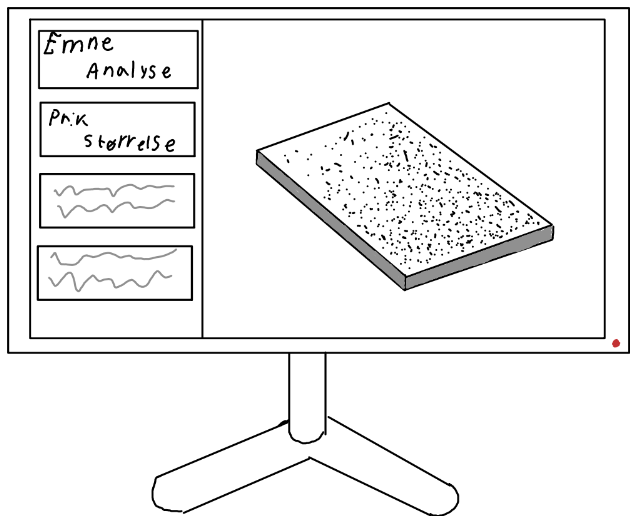
\includegraphics[width=0.98\linewidth]{Sections/5 Konceptgenerering/Media/formanalyse compu.png}} & & 19 & \makecell{\includegraphics[width=0.7\linewidth]{Sections/5 Konceptgenerering/Media/Touch skærm.png}} & \makecell{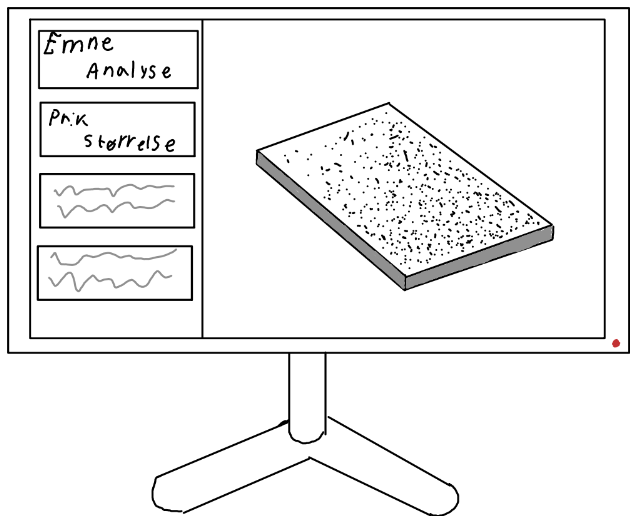
\includegraphics[width=0.98\linewidth]{Sections/5 Konceptgenerering/Media/formanalyse compu.png}}  \\ \cline{1-3} \cline{5-7}

        15 & \makecell{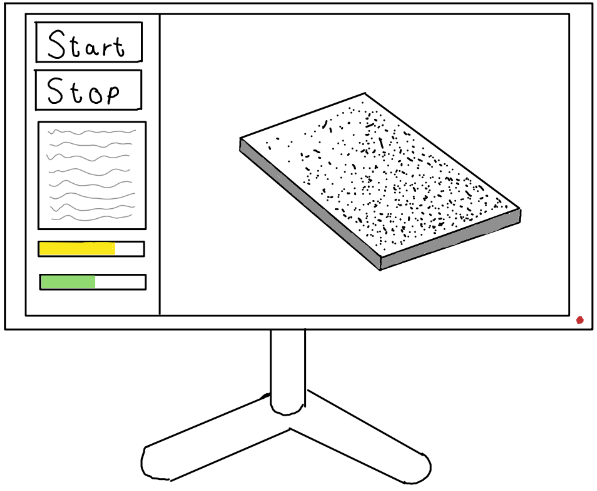
\includegraphics[width=0.7\linewidth]{Sections/5 Konceptgenerering/Media/Computer.png}} & \makecell{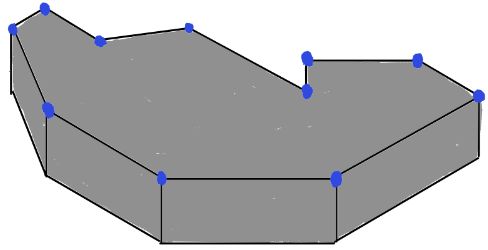
\includegraphics[width=0.98\linewidth]{Sections/5 Konceptgenerering/Media/sensor i punkt.png}} &  & 20 & \makecell{\includegraphics[width=0.7\linewidth]{Sections/5 Konceptgenerering/Media/Touch skærm.png}} & \makecell{\includegraphics[width=0.98\linewidth]{Sections/5 Konceptgenerering/Media/sensor i punkt.png}}  \\ \cline{1-3} \cline{5-7}
    \end{tabular}
\end{table}






